\documentclass{article}

\usepackage{graphicx}
\usepackage{tikz}
\usepackage{tikzsymbols}
\usetikzlibrary{calc,patterns,shapes.geometric}
\pagestyle{empty}
\usepackage[margin=0pt]{geometry}
\geometry{papersize={14in,12in}}

\def\centerarc[#1](#2)(#3:#4:#5){\draw[#1] ($(#2)+({#5*cos(#3)},{#5*sin(#3)})$) arc (#3:#4:#5);}

\begin{document}
	\begin{figure}
		\centering
		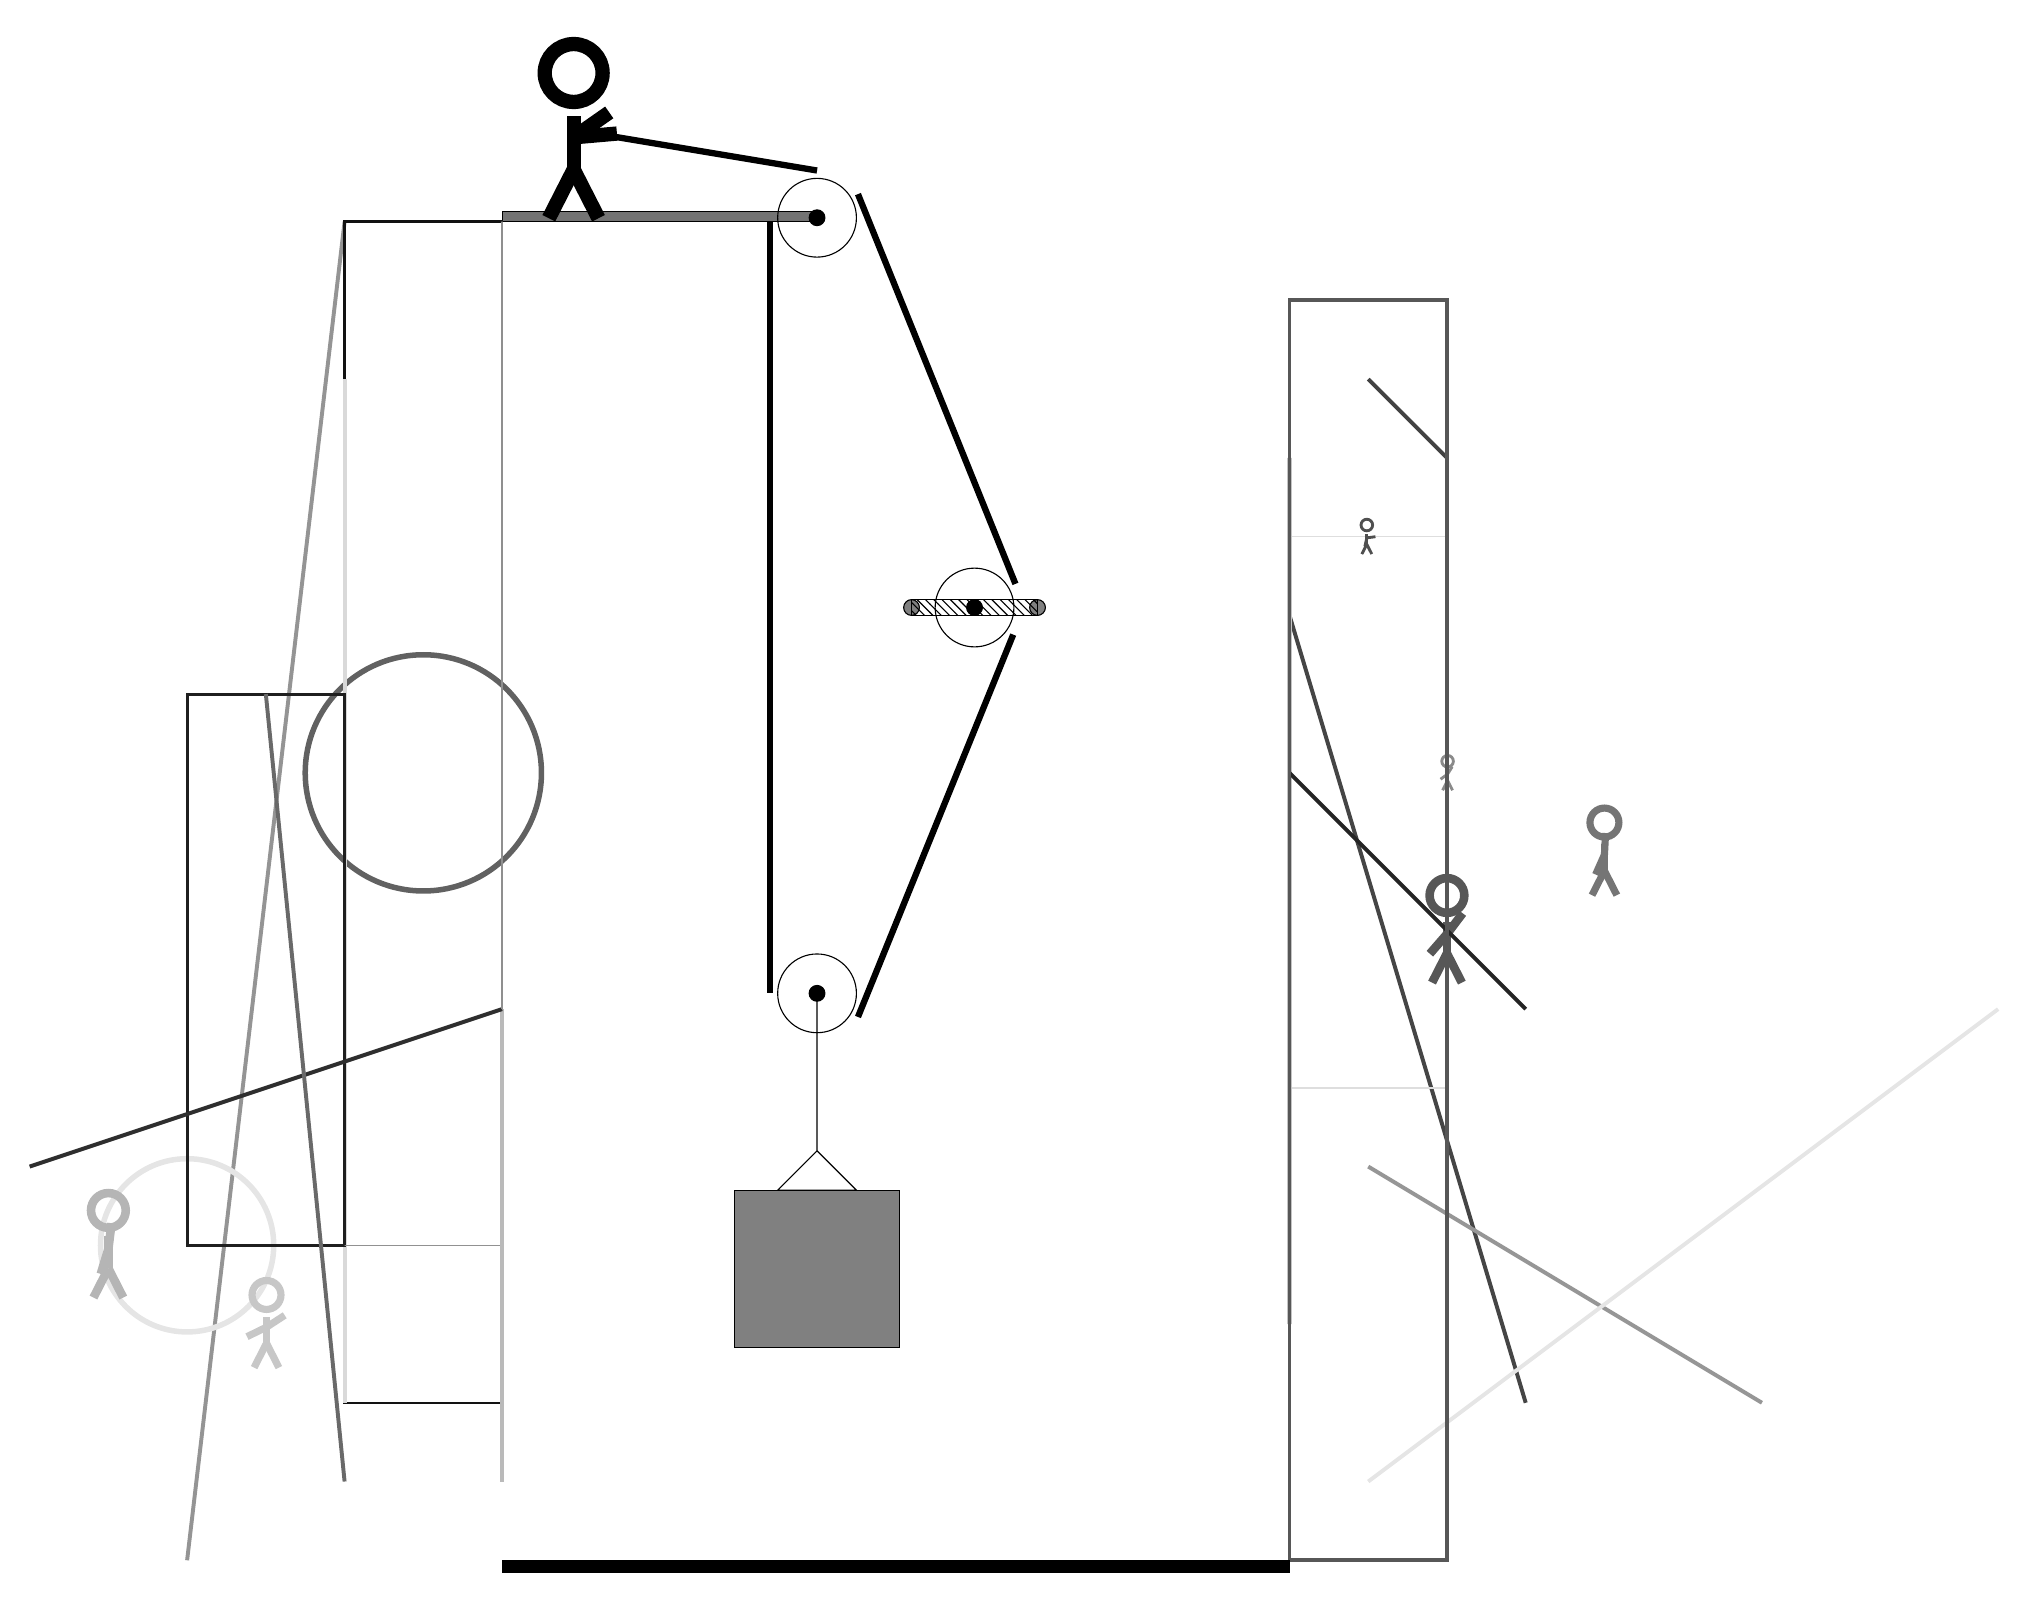
\begin{tikzpicture}
			%%%%% START %%%%%
			
			\draw[fill=black!55] (-2, 14) rectangle (2, 14.125);
			
			\draw (2, 4.2) circle (0.5);
			\draw[fill=black] (2, 4.2) circle (0.1);
			
			\draw (2, 14.05) circle (0.5);
			\draw[fill=black] (2, 14.05) circle (0.1);
			
			\draw[line width=0.5mm, color=black!74](10, 11) -- (9, 12);
			
			\draw [line width=0.7mm, color=black!62](-3, 7) circle (1.5);
			\draw[line width=0.5mm, color=black!42](-6, -3) -- (-4, 14);
			\draw [line width=0.7mm, color=black!10](-6, 1) circle (1.1);
			\node[line width=0.5mm, color=black!22] at (-5, 0) {\Strichmaxerl[5][26][33]};
			
			\draw[line width=0.5mm, color=black!73](11, -1) -- (8, 9);
			\node[line width=0.3mm, color=black!29] at (-7, 1) {\Strichmaxerl[6][73][83]};
			
			\draw[line width=0.3mm, color=black!93] (-4, 14) rectangle (-2, -1);
			\node[line width=0.5mm, color=black!46] at (10, 7) {\Strichmaxerl[2][36][58]};
			
			\draw[line width=0.2mm, color=black!13] (10, 10) rectangle (8, 3);
			\draw[line width=0.5mm, color=black!15](-4, 12) -- (-4, -1);
			
			\draw[line width=0.4mm, color=black!88] (-4, 8) rectangle (-6, 1);
			\draw[line width=0.5mm, color=black!41](9, 2) -- (14, -1);
			
			\draw[line width=0.2mm, color=black!43] (-2, 1) rectangle (-4, 1);
			\draw[line width=0.5mm, color=black!27](-2, -2) -- (-2, 4);
			\draw[line width=0.5mm, color=black!10](9, -2) -- (17, 4);
			
			\draw[line width=0.5mm, color=black!82](-2, 4) -- (-8, 2);
			
			\node[line width=0.3mm, color=black!69] at (9, 10) {\Strichmaxerl[2][77][8]};
			\draw[line width=0.2mm, color=black!44] (-2, 14) rectangle (-2, 4);
			\node[line width=0.5mm, color=black!66] at (10, 5) {\Strichmaxerl[6][49][53]};
			\draw[line width=0.6mm, color=black!53] (8, 1) rectangle (8, 8);
			\draw[line width=0.6mm, color=black!23] (8, 0) rectangle (8, 11);
			\draw[line width=0.5mm, color=black!86](8, 7) -- (11, 4);
			\draw[line width=0.5mm, color=black!59](-4, -2) -- (-5, 8);
			\node[line width=0.7mm, color=black!54] at (12, 6) {\Strichmaxerl[5][66][87]};
			\draw[line width=0.5mm, color=black!66] (10, -3) rectangle (8, 13);
			
			\draw[fill=white](4, 9.1) circle (0.5);
			\draw[fill=black] (4, 9.1) circle (0.1);
			\draw[fill=black!50] (3.2, 9.1) circle (0.1);
			\draw[fill=black!50] (4.8, 9.1) circle (0.1);
			\draw[pattern=north west lines, pattern color=black] (3.2, 9.2) rectangle (4.8, 9.0);
			
			\draw (2, 4.2) -- (2, 2.2) -- (1.5, 1.7) -- (2.5, 1.7) -- (2, 2.2);
			\draw[fill=black!50] (0.95, 1.7) rectangle (3.05, -0.3);
			
			\draw[line width=0.8mm] (1.4, 14) -- (1.4, 4.2);
			\centerarc[line width=0.8mm](2, 4.2)(180:330:0.6);
			\draw[line width=0.8mm](2.5196, 3.9) -- (4.4915, 8.7558);
			\centerarc[line width=0.8mm](4, 9.1)(390:325:0.6);
			\draw[line width=0.8mm](4.5196, 9.4) -- (2.5196, 14.35);
			\centerarc[line width=0.8mm](2, 14.05)(30:90:0.6);
			\draw[line width=0.8mm](2, 14.65) -- (-1, 15.15);
			
			\node at (-1, 15.15) {\Strichmaxerl[10][-175][35]};
			
			\draw[fill=black] (-2, -3) rectangle (8, -3.15);
			
			%%%%% END %%%%%
		\end{tikzpicture}
	\end{figure}	
\end{document}